%-------------------------------------------------------------------------------
%-------------------------------------------------------------------------------
\section{ODE en dimension 2} \label{sec:EquaDiff-nonLineaire2D}
%-------------------------------------------------------------------------------

On s'intéresse ici au cas d'une système d'ODE $\dot y = F(y)$ avec $F : \Rbb^2 \mapsto \Rbb^2$. 

%-------------------------------------------------------------------------------
\subsection{Classification des équilibres} 
%-------------------------------------------------------------------------------

La classification des équilibres repose sur l'étude des valeurs propres $\lambda_1$ et $\lambda_2$ de la matrice jacobienne $J_{y^*}$ en tout point d'équilibre $y^*$ solution de $F(y^*) = 0$. On peut ainsi définir la classification suivante :
$$
\begin{tabular}{ll}
  $(\lambda_1, \lambda_2) \in \Rbb, (\lambda_1, \lambda_2) < 0 :$ & point stable ou 'puit' ; \\
  $(\lambda_1, \lambda_2) \in \Rbb, (\lambda_1, \lambda_2) > 0 :$ & point instable ou 'source' ; \\
  $(\lambda_1, \lambda_2) \in \Rbb, \lambda_1 > 0 , \lambda_2 < 0 :$ & point selle ; \\
  $(\lambda_1, \lambda_2) \in \Cbb, \Re(\lambda_1, \lambda_2) < 0 :$ & point de concentration ou 'puit en spirale' ; \\
  $(\lambda_1, \lambda_2) \in \Cbb, \Re(\lambda_1, \lambda_2) > 0 :$ & point de repulsion ou 'source en spirale'. \\
  $(\lambda_1, \lambda_2) \in \Cbb \setminus \Rbb:$ & voir ci-dessous.
\end{tabular}
$$

\begin{figure}[ht]
  \begin{center}
    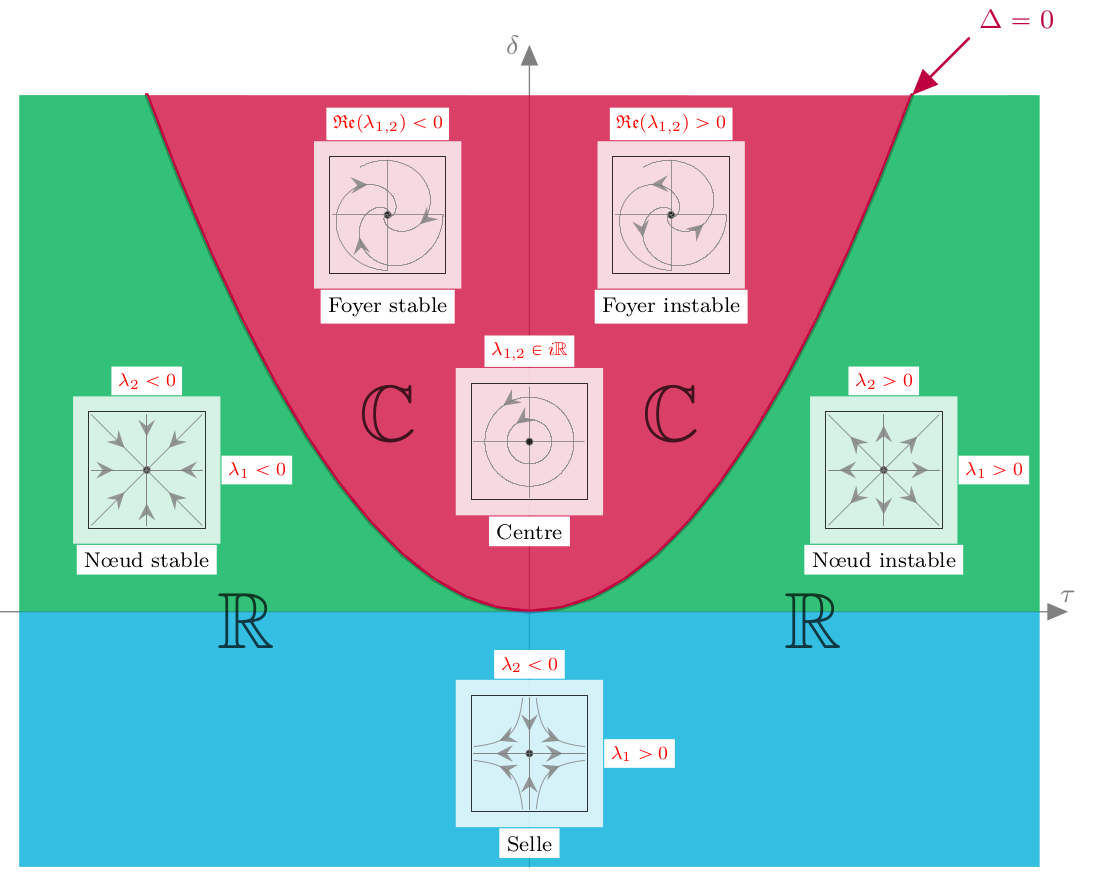
\includegraphics{L3-SU-MathBio-StabiliteEquilibresD2}
  \end{center}
  \caption{Stabilité des équilibres en dimension 2. $\tau = \tr(A)$, $\delta=|A|$, $\Delta = \tau^2 - 4 \delta$ (discriminant de $P_A(\lambda)$.}
\end{figure}

Les théorèmes vus jusqu'à présent ne permettent pas d'étudier le dernier cas, qui correspond à des trajectoires limites cycliques.

%-------------------------------------------------------------------------------
\subsection{Existence d'orbites périodiques} 
%-------------------------------------------------------------------------------

\begin{definition}[Orbite]
  Pour toute solution $(f, I)$ d'une ODE, on appelle \emph{orbite} l'ensemble $\{f(t), t \in I\}$. S'il existe $t_0$ tel que $[t_0, \infty) \subset I$, l'ensemble $\{f(t), t \geq t_0\}$ est appelé \emph{semi-orbite positive}.
\end{definition}

%-------------------------------------------------------------------------------
\begin{theorem}[Poincarré-Bendixson]
  Soit $D$ un fermé borné de $\Rbb^2$ ne contenant pas de point d'équilibre d'une ODE $\dot y = F(y)$. S'il existe une semi-orbite positive $O$ entièrement comprise dans $D$ alors l'ensemble $C$ des points limite de $O$ est une orbite périodique. Si $O$ n'est pas l'ensemble $C$, $C$ et appelé cycle limite.
\end{theorem}

\remark
Le théorème dit que si une trajectoire solution de l'ODE est piégée dans une région $D$ bornée de $\Rbb^2$, elle doit se rapprocher de plus en plus d'une courbe $C$ fermée. Il n'est souvent pas difficile d'identifier une telle région $D$, mais déterminer le cycle limite $C$ est souvent plus difficile.

%-------------------------------------------------------------------------------
\paragraph*{Détermination d'un cycle.} 

\begin{definition}[Hamiltionien]
  Un hamiltionien (ou une fonction hamiltonienne) d'une ODE est une fonction $H : \Rbb^n \mapsto \Rbb$ qui reste constante le long des trajectoires solution de l'ODE.
\end{definition}

\remark
Cette définition revient à dire que les solutions $y(t)$ suivent des lignes de niveau de la fonction hamiltonienne.

\bigskip
\begin{proposition}[Hamiltionien] \label{prop:hamiltonien}
  Si $H$ est un hamiltonien de l'EDO $\{\dot y = F(y), y(0) = y_0\}$, où $F$ est une application de $\Rbb^n$ dans $\Rbb^n$, il vérifie :
  $$
  \sum_{i=1}^n F_i(y) \left.\frac{\partial H}{\partial y_i}\right|_{y(t)} = 0.
  $$
\end{proposition}

% {Démonstration de la proposition \ref{prop:hamiltonien}.}
\proof
  La définition du hamiltonien impose que 
  $$
  \frac{\partial}{\partial t} H(y(t)) \equiv 0.
  $$
  Pour déterminer la dérivée de $H(y(t))$ par rapport au temps, on utilise la proposition \ref{prop:compositionDifferentielles} avec $f = H$ et $g = y$, soit
%   $$
%   \begin{array}{rrcl}
%     f : & \Rbb^n & \mapsto & \Rbb \\
%     & y & \to & f(y) = H(y)
%   \end{array},
%   \qquad
%   \begin{array}{rrcl}
%     g : & \Rbb & \mapsto & \Rbb^n \\
%     & t & \to & g(y) = y(t)
%   \end{array},
%   $$
%   soit
  $$
  \frac{\partial}{\partial t} H(y(t)) 
  = J_{y(t)}H \cdot J_ty
  $$
  où
  $$
  J_{y(t)}H = \left[ \begin{array}{ccc}
    \displaystyle{\left.\frac{\partial H}{\partial y_1}\right|_{y(t)}} & 
    \dots & 
    \displaystyle{\left.\frac{\partial H}{\partial y_n}\right|_{y(t)}} 
  \end{array}\right] 
  \qquad \text{et} \qquad 
  J_ty = \left[\begin{array}{c} 
    \dot y_1(t) = F_1(y(t)) \\
    \vdots \\
    \dot y_1(t) = F_n(y(t))
  \end{array}\right] 
  $$
\eproof

%-------------------------------------------------------------------------------
\paragraph*{Cas $n = 2$.} 
On considère une ODE avec $F : \Rbb^2 \mapsto \Rbb^2$ : 
$$
\left\{\begin{array}{rcl} \dot x & = & F_1(x, y) \\ \dot y & = & F_2(x, y) \end{array}\right.
$$
Soit $(x(t), y(t))$ une solution maximale sur $I$ pour la condition initiales $(x(t_0), y(t_0)) = (x_0, y_0)$. Un hamitonien est une fonction $H : \Rbb^2 \mapsto \Rbb^2$ qui vérifie
$$
\forall t \in I: \quad H(x(t), y(t)) = H(x_0, y_0).
$$
Les orbites sont alors les lignes de niveau du hamiltonien : 
$$
\Ccal_z = \{x, y: H(x, y) = z\}.
$$

La difficulté réside alors dans la détermination d'une fonction $H$ qui vérifie la proposition \ref{prop:hamiltonien} en dimension 2. En appliquant la règle de composition $J_x f \circ g = J_{g(x)} f \; J_x g$, il vient : 
\begin{align} \label{eq:derivHnulleD2}
  \dot H(x, y) =
  \frac{\partial H}{\partial x} (x(t), y(t)) \dot x(t) +
  \frac{\partial H}{\partial y} (x(t), y(t)) \dot y(t) & = 0 \nonumber \\
  \Leftrightarrow \qquad 
  F_1(x, y) \frac{\partial H}{\partial x} (x, y) +
  F_2(x, y) \frac{\partial H}{\partial y} (x, y) & = 0.
\end{align}

%-------------------------------------------------------------------------------
\paragraph*{Cas ``séparable''.} 
On peut chercher une fonction $H$ séparable, c'est-à-dire de la forme
$$
H(x, y) = h_1(x) + h_2(y).
$$
On a alors
$$
\frac{\partial H}{\partial x} = h_1'(x), \qquad
\frac{\partial H}{\partial y} = h_2'(x)
$$
et la condition \eqref{eq:derivHnulleD2} devient
$$
F_1(x, y) h_1'(x) = -F_2(x, y) h_2'(y)
\qquad \Leftrightarrow \qquad
\frac{F_1(x, y)}{F_2(x, y)} = -\frac{h_2'(y)}{h_1'(x)}.
$$
On peut donc déterminer un hamiltonien de la forme $H(x, y) = h_1(x) + h_2(y)$ si on peut trouver $f$ et $g$ telles que
$$
\frac{F_1(x, y)}{F_2(x, y)} = \frac{g(y)}{f(x)}.
$$
Il reste alors à déterminer des fonctions $h_1$ et $h_2$ satisfaisant
$$
h'_1(x) = k f(x), \qquad
h'_2(y) = - k g(y).
$$
On utilisera cette méthode pour caractériser les cycles du modèle de Lotka-Volterra.
